%----------------------------------------------------------------------------
\label{computer chapter}
%----------------------------------------------------------------------------
%%%%%%%%%%%%%%%%%%%%%%%%%%%%%% -*- Mode: Latex -*- %%%%%%%%%%%%%%%%%%%%%%%%%%%%
%% >>slacT486/intro.tex<<
%% Author          : R. Jeffrey Kowalski
%% Created On      : Tue Apr 10 19:50:51 HST 2007
%% Last Modified On: Thu Aug  2 10:54:56 HST 2007
%%%%%%%%%%%%%%%%%%%%%%%%%%%%%%%%%%%%%%%%%%%%%%%%%%%%%%%%%%%%%%%%%%%%%%%%%%%%%%%
From June 19-24, 2006, the experiment, SLAC T486, was performed in the End Station A facility at the Stanford Linear Accelerator Center to measure the Askaryan effect in ice.  28.5 GeV electrons were accelerated with typically 10$^9$ particles in 10 picosecond bunches and delivered into a 7.5 metric tonne target of carving-grade ice to produce electromagnetic showers.  In a dense media like ice, coherent microwave Cherenkov radiation emerges from the particle shower and propagates to the surface of the target where radio antennas can detect the radiation.  This chapter outlines the T486 experiment and the analysis of the Askaryan effect in ice.
%----------------------------------------------------------------------------
%----------------------------------------------------------------------------
\section{Transform limited pulse sequences}
%----------------------------------------------------------------------------
%----------------------------------------------------------------------------
\subsection{One color}
%----------------------------------------------------------------------------
%----------------------------------------------------------------------------
%----------------------------------------------------------------------------
Suppose the dynamics of some two level quantum system is given by
%----------------------------------------------------------------------------
\begin{equation}
i\frac{\partial}{\partial t} \ket{\Psi}
=
i\left(
\begin{array}{cc}
0 & \alpha \\
-\alpha & 0 \\
\end{array}
\right)
\ket{\Psi},
\label{one dynamics}
\end{equation}
%----------------------------------------------------------------------------
where the square of the nth element in $\ket{\Psi}$ is the probability of finding the system in the nth state, $\alpha$ is the coupling field between the zeroth (ground) and first excited state. It can be shown (see Section \ref{basic_two_level}) that closed non-degenerate two level quantum systems with a completely resonant coupling field can be described this way in the energy basis (see Figure \ref{1 color ladder}).
%----------------------------------------------------------------------------
%----------------------------------------------------------------------------
% 1_color_ladder.tex
% by Troy Hix, April 2005
%----------------------------------------------------------------------------
%----------------------------------------------------------------------------
\begin{figure}[h]
\setlength{\unitlength}{2cm}
\begin{center}
\begin{picture}(3.3,2.2)
\linethickness{1mm}
\put(0,1.2){\line(1,0){3}}
\put(0,0.0){\line(1,0){3}}
\put(3.1,1.2){$\ket{1}$}
\put(3.1,0.0){$\ket{0}$}
\thinlines
\put(1.0,0.0){\vector(0,1){1.18}}
\put(1.2,0.6){$\alpha$}
\end{picture}
\end{center}
\caption[Two level, single field diagram]{Two level, single field diagram. Ground state $\ket{0}$ and first excited state $\ket{1}$ are coupled by field $\alpha$ so that population transfers from the ground state to the first excited state}
\label{1 color ladder}
\end{figure}
%----------------------------------------------------------------------------
%----------------------------------------------------------------------------

%----------------------------------------------------------------------------
%----------------------------------------------------------------------------
%----------------------------------------------------------------------------
%----------------------------------------------------------------------------
%----------------------------------------------------------------------------
In general the coupling field is a function of time. Consider solutions where the coupling field is localized temporally as a Gaussian, namely
%----------------------------------------------------------------------------
\begin{equation}
\boxed{
\alpha(t)
=
A
\exp
\left(
-\ln(16)
\frac
{(t - t_\alpha)^2}
{\sigma_\alpha^2}
\right),
\label{gaussian}
}
\end{equation}
%----------------------------------------------------------------------------
where $A$ is the amplitude, $t_\alpha$ is location of the pulse, $\sigma_\alpha$ is the full width half max (FWHM) of the pulse amplitude.

%----------------------------------------------------------------------------
%----------------------------------------------------------------------------

%----------------------------------------------------------------------------
%----------------------------------------------------------------------------
% solution_3_pulses.tex
% by Troy Hix, March 2005
%----------------------------------------------------------------------------
\begin{figure}
\centering
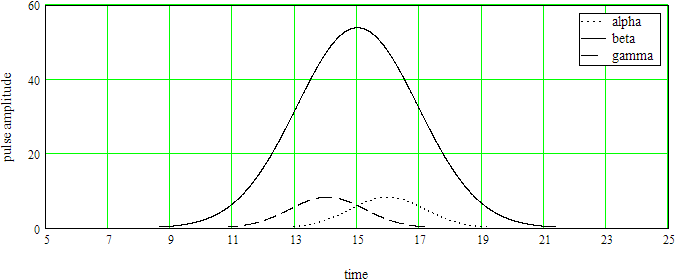
\includegraphics[width=5.00in]
{solution_3_pulses/solution_3_pulses.png}\\
\caption[Three color optimal pulse sequence]{Three color optimal pulse sequence. When $w=10^8$, the local optimum occurs when $\sigma_\alpha=\sigma_\gamma=2.84885872022$, $\sigma_\beta=4.59093152823$, $A=C=8.28793940926$ (5.093 times the area of the $\pi$--pulse), $B=53.8858080585$ (53.363 times the area of the $\pi$--pulse), and $\Delta_\alpha=\Delta_\gamma=-0.972655687674$.}
\label{solution three pulses}
\end{figure} 
%----------------------------------------------------------------------------

%----------------------------------------------------------------------------
%----------------------------------------------------------------------------
Suppose the solution, $\ket{\Psi}$, to (\ref{one dynamics}) is known at N+1 points from $t_0$ to $t_N$ where $t_i<t_j$ when $i<j$ $\forall$  $i,j \in \{0,1,\cdots,N\}$. Let $\ket{n}_i$ be the value of the nth component ($n \in \{ 0,1,2,3 \}$) of the solution, $\ket{\Psi}$, at time $t_i$. Consider the cost function
%----------------------------------------------------------------------------
%----------------------------------------------------------------------------
\begin{equation}
\Phi
=
w\Phi_{residue}
+
\Phi_{intermediate}
\label{three cost}
\end{equation}
%----------------------------------------------------------------------------
where
%----------------------------------------------------------------------------
\begin{equation}
\Phi_{residue}
=
P_0(t_N)
+
P_1(t_N)
+
P_2(t_N)
\label{three residue cost}
\end{equation}
%----------------------------------------------------------------------------
%----------------------------------------------------------------------------
% solution_3_energy_levels.tex
% by Troy Hix, April 2005
%----------------------------------------------------------------------------
\begin{figure}
\centering
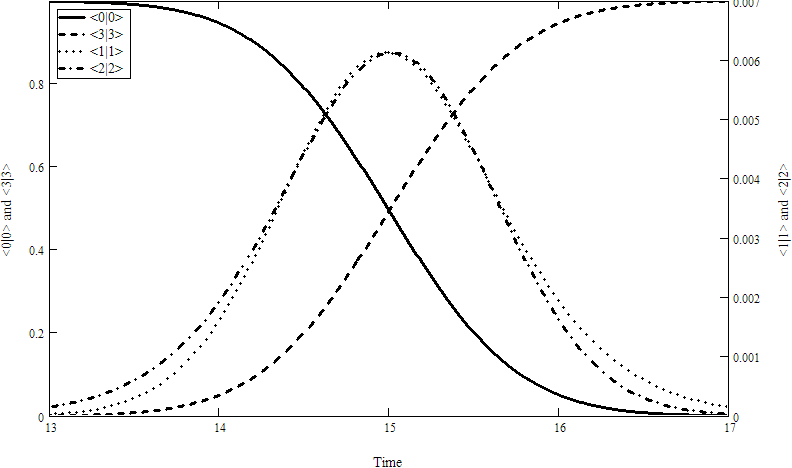
\includegraphics[width=5.00in]
{solution_3_energy_levels/solution_3_energy_levels.png}\\
\caption[Three color optimal solution]{Three color optimal solution. Occupation probability of the intermediate states $\ket{1}$ and $\ket{2}$ remain small while states $\ket{0}$ and $\ket{3}$ essentially exchange unity occupation probability in what looks like a single color $\pi$-pulse process (see figure \ref{solution one}).}
\label{solution three energy levels}
\end{figure} 
%----------------------------------------------------------------------------

%----------------------------------------------------------------------------
%----------------------------------------------------------------------------
\begin{equation}
\Phi_{intermediate}
=
\sum_i^N
P_1(t_i)
+
P_2(t_i)
\label{three int cost}
\end{equation}
%----------------------------------------------------------------------------
and $w$ is some weight factor.
%----------------------------------------------------------------------------
%----------------------------------------------------------------------------
A MathCAD program was written to minimize (\ref{three cost}) as a function of $\sigma_\alpha$, $\sigma_\beta$, $\sigma_\gamma$, $A$, $B$, $C$, $\Delta_\alpha$ and $\Delta_\gamma$. After some initial runs, some symmetries in the solutions prompted the following reduction of variables: $\sigma_\alpha=\sigma_\gamma$, $A=C$, $\Delta_\alpha=\Delta_\gamma$. Figure \ref{solution three pulses} shows the pulse sequence which minimized the cost function and figure \ref{solution three energy levels} shows the resulting motion in $\braket{\Psi}{\Psi}$.

In general, there are many local optima in the five dimensional solution space. It was found (with some exploring) that these optima generally improve with increasing amplitudes $A$, $B$, and $C$. Figure \ref{big solution three energy levels} show an example of one such solution. Note again the ``counter--intuitive'' pulse order of the first and last pulse.
%----------------------------------------------------------------------------
%----------------------------------------------------------------------------
% big_solution_3_energy_levels.tex
% by Troy Hix, April 2005
%----------------------------------------------------------------------------
\begin{figure}
\centering
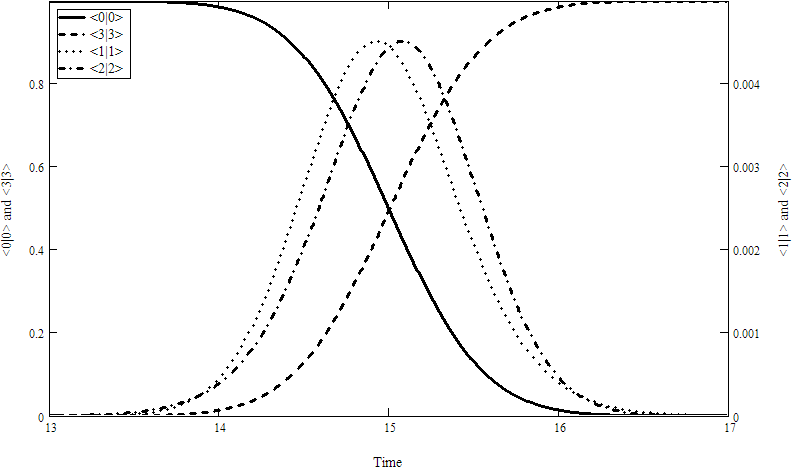
\includegraphics[width=5.00in]
{big_solution_3_energy_levels/big_solution_3_energy_levels.png}\\
\caption[Three color optimal solution - increased pulse amplitude]{Three color optimal solution - increased pulse amplitude. The local optimum ($w=10^8$) occurs when $\sigma_\alpha=\sigma_\gamma=2.19612383897$, $\sigma_\beta=4.57812933276$, $A=C=15.8819988348$ (7.524 times the area of the $\pi$--pulse), $B=101.198555496$ (99.937 times the area of the $\pi$--pulse), and $\Delta_\alpha=\Delta_\gamma=-0.93886228288$.}
\label{big solution three energy levels}
\end{figure} 
%----------------------------------------------------------------------------

%----------------------------------------------------------------------------
%----------------------------------------------------------------------------
%----------------------------------------------------------------------------

%----------------------------------------------------------------------------
%----------------------------------------------------------------------------
\subsection{Two color}
%----------------------------------------------------------------------------
%----------------------------------------------------------------------------
%----------------------------------------------------------------------------
Suppose the dynamics of some two level quantum system is given by
%----------------------------------------------------------------------------
\begin{equation}
i\frac{\partial}{\partial t} \ket{\Psi}
=
i\left(
\begin{array}{cc}
0 & \alpha \\
-\alpha & 0 \\
\end{array}
\right)
\ket{\Psi},
\label{one dynamics}
\end{equation}
%----------------------------------------------------------------------------
where the square of the nth element in $\ket{\Psi}$ is the probability of finding the system in the nth state, $\alpha$ is the coupling field between the zeroth (ground) and first excited state. It can be shown (see Section \ref{basic_two_level}) that closed non-degenerate two level quantum systems with a completely resonant coupling field can be described this way in the energy basis (see Figure \ref{1 color ladder}).
%----------------------------------------------------------------------------
%----------------------------------------------------------------------------
% 1_color_ladder.tex
% by Troy Hix, April 2005
%----------------------------------------------------------------------------
%----------------------------------------------------------------------------
\begin{figure}[h]
\setlength{\unitlength}{2cm}
\begin{center}
\begin{picture}(3.3,2.2)
\linethickness{1mm}
\put(0,1.2){\line(1,0){3}}
\put(0,0.0){\line(1,0){3}}
\put(3.1,1.2){$\ket{1}$}
\put(3.1,0.0){$\ket{0}$}
\thinlines
\put(1.0,0.0){\vector(0,1){1.18}}
\put(1.2,0.6){$\alpha$}
\end{picture}
\end{center}
\caption[Two level, single field diagram]{Two level, single field diagram. Ground state $\ket{0}$ and first excited state $\ket{1}$ are coupled by field $\alpha$ so that population transfers from the ground state to the first excited state}
\label{1 color ladder}
\end{figure}
%----------------------------------------------------------------------------
%----------------------------------------------------------------------------

%----------------------------------------------------------------------------
%----------------------------------------------------------------------------
%----------------------------------------------------------------------------
%----------------------------------------------------------------------------
%----------------------------------------------------------------------------
In general the coupling field is a function of time. Consider solutions where the coupling field is localized temporally as a Gaussian, namely
%----------------------------------------------------------------------------
\begin{equation}
\boxed{
\alpha(t)
=
A
\exp
\left(
-\ln(16)
\frac
{(t - t_\alpha)^2}
{\sigma_\alpha^2}
\right),
\label{gaussian}
}
\end{equation}
%----------------------------------------------------------------------------
where $A$ is the amplitude, $t_\alpha$ is location of the pulse, $\sigma_\alpha$ is the full width half max (FWHM) of the pulse amplitude.

%----------------------------------------------------------------------------
%----------------------------------------------------------------------------

%----------------------------------------------------------------------------
%----------------------------------------------------------------------------
% solution_3_pulses.tex
% by Troy Hix, March 2005
%----------------------------------------------------------------------------
\begin{figure}
\centering
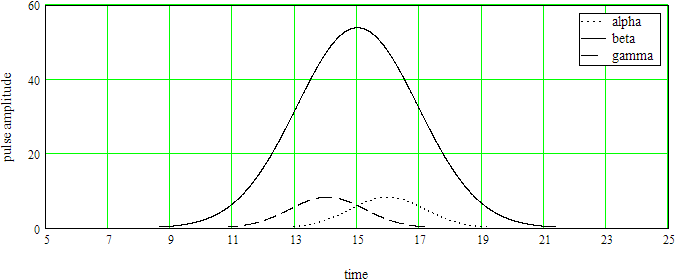
\includegraphics[width=5.00in]
{solution_3_pulses/solution_3_pulses.png}\\
\caption[Three color optimal pulse sequence]{Three color optimal pulse sequence. When $w=10^8$, the local optimum occurs when $\sigma_\alpha=\sigma_\gamma=2.84885872022$, $\sigma_\beta=4.59093152823$, $A=C=8.28793940926$ (5.093 times the area of the $\pi$--pulse), $B=53.8858080585$ (53.363 times the area of the $\pi$--pulse), and $\Delta_\alpha=\Delta_\gamma=-0.972655687674$.}
\label{solution three pulses}
\end{figure} 
%----------------------------------------------------------------------------

%----------------------------------------------------------------------------
%----------------------------------------------------------------------------
Suppose the solution, $\ket{\Psi}$, to (\ref{one dynamics}) is known at N+1 points from $t_0$ to $t_N$ where $t_i<t_j$ when $i<j$ $\forall$  $i,j \in \{0,1,\cdots,N\}$. Let $\ket{n}_i$ be the value of the nth component ($n \in \{ 0,1,2,3 \}$) of the solution, $\ket{\Psi}$, at time $t_i$. Consider the cost function
%----------------------------------------------------------------------------
%----------------------------------------------------------------------------
\begin{equation}
\Phi
=
w\Phi_{residue}
+
\Phi_{intermediate}
\label{three cost}
\end{equation}
%----------------------------------------------------------------------------
where
%----------------------------------------------------------------------------
\begin{equation}
\Phi_{residue}
=
P_0(t_N)
+
P_1(t_N)
+
P_2(t_N)
\label{three residue cost}
\end{equation}
%----------------------------------------------------------------------------
%----------------------------------------------------------------------------
% solution_3_energy_levels.tex
% by Troy Hix, April 2005
%----------------------------------------------------------------------------
\begin{figure}
\centering
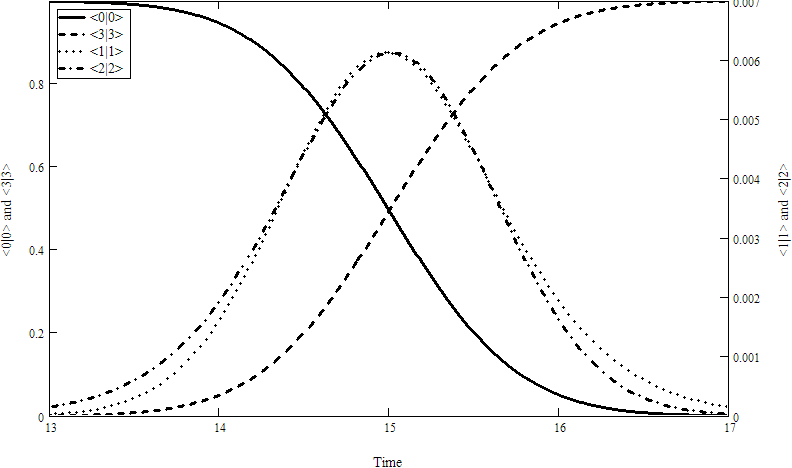
\includegraphics[width=5.00in]
{solution_3_energy_levels/solution_3_energy_levels.png}\\
\caption[Three color optimal solution]{Three color optimal solution. Occupation probability of the intermediate states $\ket{1}$ and $\ket{2}$ remain small while states $\ket{0}$ and $\ket{3}$ essentially exchange unity occupation probability in what looks like a single color $\pi$-pulse process (see figure \ref{solution one}).}
\label{solution three energy levels}
\end{figure} 
%----------------------------------------------------------------------------

%----------------------------------------------------------------------------
%----------------------------------------------------------------------------
\begin{equation}
\Phi_{intermediate}
=
\sum_i^N
P_1(t_i)
+
P_2(t_i)
\label{three int cost}
\end{equation}
%----------------------------------------------------------------------------
and $w$ is some weight factor.
%----------------------------------------------------------------------------
%----------------------------------------------------------------------------
A MathCAD program was written to minimize (\ref{three cost}) as a function of $\sigma_\alpha$, $\sigma_\beta$, $\sigma_\gamma$, $A$, $B$, $C$, $\Delta_\alpha$ and $\Delta_\gamma$. After some initial runs, some symmetries in the solutions prompted the following reduction of variables: $\sigma_\alpha=\sigma_\gamma$, $A=C$, $\Delta_\alpha=\Delta_\gamma$. Figure \ref{solution three pulses} shows the pulse sequence which minimized the cost function and figure \ref{solution three energy levels} shows the resulting motion in $\braket{\Psi}{\Psi}$.

In general, there are many local optima in the five dimensional solution space. It was found (with some exploring) that these optima generally improve with increasing amplitudes $A$, $B$, and $C$. Figure \ref{big solution three energy levels} show an example of one such solution. Note again the ``counter--intuitive'' pulse order of the first and last pulse.
%----------------------------------------------------------------------------
%----------------------------------------------------------------------------
% big_solution_3_energy_levels.tex
% by Troy Hix, April 2005
%----------------------------------------------------------------------------
\begin{figure}
\centering
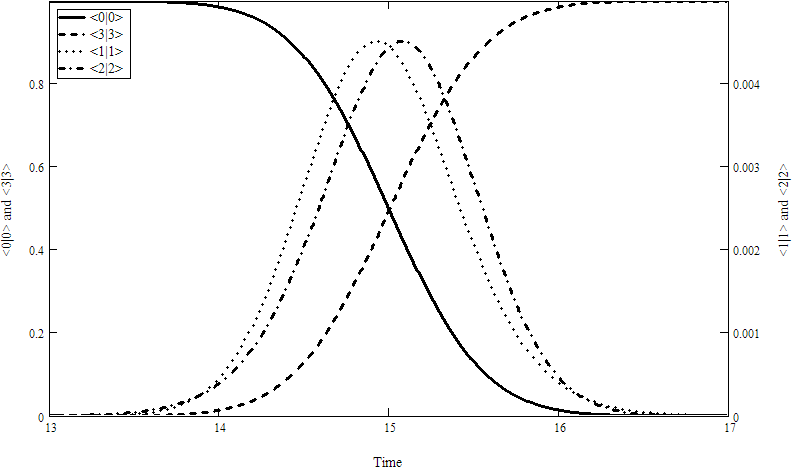
\includegraphics[width=5.00in]
{big_solution_3_energy_levels/big_solution_3_energy_levels.png}\\
\caption[Three color optimal solution - increased pulse amplitude]{Three color optimal solution - increased pulse amplitude. The local optimum ($w=10^8$) occurs when $\sigma_\alpha=\sigma_\gamma=2.19612383897$, $\sigma_\beta=4.57812933276$, $A=C=15.8819988348$ (7.524 times the area of the $\pi$--pulse), $B=101.198555496$ (99.937 times the area of the $\pi$--pulse), and $\Delta_\alpha=\Delta_\gamma=-0.93886228288$.}
\label{big solution three energy levels}
\end{figure} 
%----------------------------------------------------------------------------

%----------------------------------------------------------------------------
%----------------------------------------------------------------------------
%----------------------------------------------------------------------------

%----------------------------------------------------------------------------

For the optimal solution, $\Phi_{residue}=9\cross10^{-15}$, we map out the surface this variable defines in solution space using two coordinate systems.
%----------------------------------------------------------------------------
%----------------------------------------------------------------------------
The region in solution space near the optimal solution shown in Figure \ref{solution 2 pulses} was mapped out by allowing the magnitude of $\Delta_{\alpha}$ and $A$ to vary by $\pm 50\%$. Figure \ref{delay amp} shows the resulting $\log(\Psi_{residue})$ surface.
%----------------------------------------------------------------------------
%----------------------------------------------------------------------------
The region in solution space near the optimal solution shown in Figure \ref{solution 2 pulses} was mapped out by allowing the magnitude of $A$ and $B$ to vary by $\pm 50\%$. Figure \ref{amp amp} shows the resulting $\log(\Psi_{residue})$ surface. Figures \ref{delay amp} and \ref{amp amp} show the robustness of the STIRAP process with regards to population transfer. The since the residue is less than $10^{-2}$ for most of the points (i.e. there is very little population left over in states 0 and 1) population transfer in nearly complete for relatively large detuning of certain pulse parameters (amplitude and delay). This means that even if there are fluctuations in these parameters, the targeted two color pathway will still result in nearly complete population transfer; thus the probability that the final target state releases a fluorescence photon is nearly independent of these types of fluctuations.
%----------------------------------------------------------------------------
%----------------------------------------------------------------------------
% delay_amp.tex
% by Troy Hix, March 2005
%----------------------------------------------------------------------------
\begin{figure}
\centering
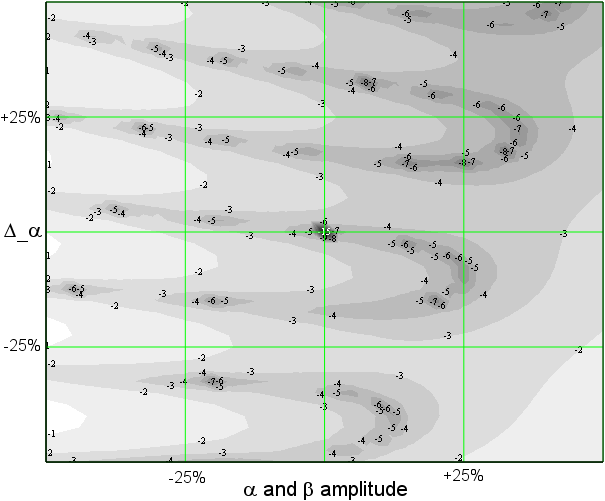
\includegraphics[width=4.00in]
{delay_amp/delay_amp.png}\\
\caption[$\log\left(\Phi_{residue}\right)$ dependence on scaling $\Delta_{\alpha}$ and $A$]{$\log\left(\Phi_{residue}\right)$ dependence on scaling $\Delta_{\alpha}$ and $A$. There are many local optima arranged in a repeating crescent shape. In general the local optima and the average height of the nearby surface decreases as $\Delta_{\alpha}$ and $A$ increase. There are $41^2$ evenly spaced points here.}
\label{delay amp}
\end{figure} 
%----------------------------------------------------------------------------

%----------------------------------------------------------------------------
%----------------------------------------------------------------------------
% amp_amp.tex
% by Troy Hix, March 2005
%----------------------------------------------------------------------------
\begin{figure}
\centering
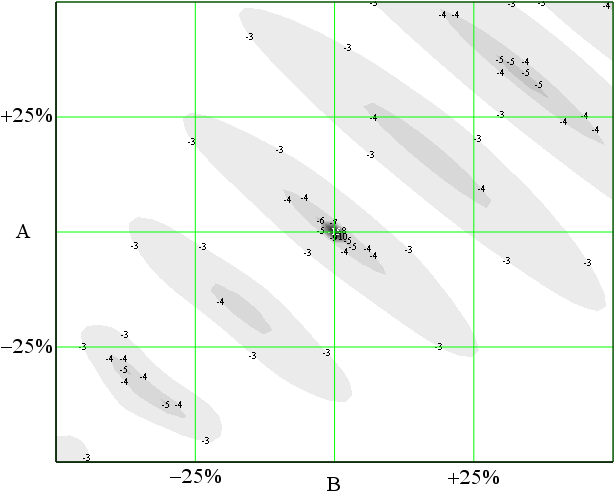
\includegraphics[width=4.00in]
{amp_amp/amp_amp.png}\\
\caption[$\Phi_{residue}$ dependence on scaling $A$ and $B$]{$\Phi_{residue}$ dependence on scaling $A$ and $B$. There are many local optima along the line defined by $A=B$. These optima improve as amplitudes $A$ and $B$ increase; and, in general, the surface slopes down as $A$ and $B$ increase. There are $41^2$ evenly spaced points here.}
\label{amp amp}
\end{figure} 
%----------------------------------------------------------------------------

%----------------------------------------------------------------------------
%----------------------------------------------------------------------------

%----------------------------------------------------------------------------
%----------------------------------------------------------------------------
\subsection{Three color}
%----------------------------------------------------------------------------
%----------------------------------------------------------------------------
%----------------------------------------------------------------------------
Suppose the dynamics of some two level quantum system is given by
%----------------------------------------------------------------------------
\begin{equation}
i\frac{\partial}{\partial t} \ket{\Psi}
=
i\left(
\begin{array}{cc}
0 & \alpha \\
-\alpha & 0 \\
\end{array}
\right)
\ket{\Psi},
\label{one dynamics}
\end{equation}
%----------------------------------------------------------------------------
where the square of the nth element in $\ket{\Psi}$ is the probability of finding the system in the nth state, $\alpha$ is the coupling field between the zeroth (ground) and first excited state. It can be shown (see Section \ref{basic_two_level}) that closed non-degenerate two level quantum systems with a completely resonant coupling field can be described this way in the energy basis (see Figure \ref{1 color ladder}).
%----------------------------------------------------------------------------
%----------------------------------------------------------------------------
% 1_color_ladder.tex
% by Troy Hix, April 2005
%----------------------------------------------------------------------------
%----------------------------------------------------------------------------
\begin{figure}[h]
\setlength{\unitlength}{2cm}
\begin{center}
\begin{picture}(3.3,2.2)
\linethickness{1mm}
\put(0,1.2){\line(1,0){3}}
\put(0,0.0){\line(1,0){3}}
\put(3.1,1.2){$\ket{1}$}
\put(3.1,0.0){$\ket{0}$}
\thinlines
\put(1.0,0.0){\vector(0,1){1.18}}
\put(1.2,0.6){$\alpha$}
\end{picture}
\end{center}
\caption[Two level, single field diagram]{Two level, single field diagram. Ground state $\ket{0}$ and first excited state $\ket{1}$ are coupled by field $\alpha$ so that population transfers from the ground state to the first excited state}
\label{1 color ladder}
\end{figure}
%----------------------------------------------------------------------------
%----------------------------------------------------------------------------

%----------------------------------------------------------------------------
%----------------------------------------------------------------------------
%----------------------------------------------------------------------------
%----------------------------------------------------------------------------
%----------------------------------------------------------------------------
In general the coupling field is a function of time. Consider solutions where the coupling field is localized temporally as a Gaussian, namely
%----------------------------------------------------------------------------
\begin{equation}
\boxed{
\alpha(t)
=
A
\exp
\left(
-\ln(16)
\frac
{(t - t_\alpha)^2}
{\sigma_\alpha^2}
\right),
\label{gaussian}
}
\end{equation}
%----------------------------------------------------------------------------
where $A$ is the amplitude, $t_\alpha$ is location of the pulse, $\sigma_\alpha$ is the full width half max (FWHM) of the pulse amplitude.

%----------------------------------------------------------------------------
%----------------------------------------------------------------------------

%----------------------------------------------------------------------------
%----------------------------------------------------------------------------
% solution_3_pulses.tex
% by Troy Hix, March 2005
%----------------------------------------------------------------------------
\begin{figure}
\centering
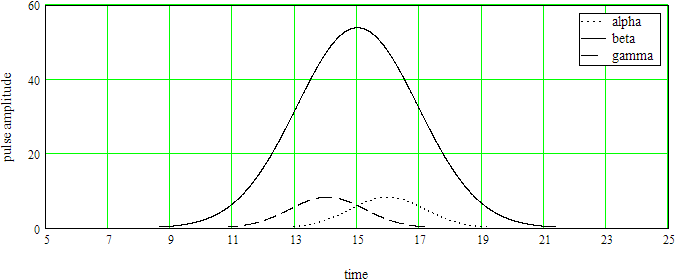
\includegraphics[width=5.00in]
{solution_3_pulses/solution_3_pulses.png}\\
\caption[Three color optimal pulse sequence]{Three color optimal pulse sequence. When $w=10^8$, the local optimum occurs when $\sigma_\alpha=\sigma_\gamma=2.84885872022$, $\sigma_\beta=4.59093152823$, $A=C=8.28793940926$ (5.093 times the area of the $\pi$--pulse), $B=53.8858080585$ (53.363 times the area of the $\pi$--pulse), and $\Delta_\alpha=\Delta_\gamma=-0.972655687674$.}
\label{solution three pulses}
\end{figure} 
%----------------------------------------------------------------------------

%----------------------------------------------------------------------------
%----------------------------------------------------------------------------
Suppose the solution, $\ket{\Psi}$, to (\ref{one dynamics}) is known at N+1 points from $t_0$ to $t_N$ where $t_i<t_j$ when $i<j$ $\forall$  $i,j \in \{0,1,\cdots,N\}$. Let $\ket{n}_i$ be the value of the nth component ($n \in \{ 0,1,2,3 \}$) of the solution, $\ket{\Psi}$, at time $t_i$. Consider the cost function
%----------------------------------------------------------------------------
%----------------------------------------------------------------------------
\begin{equation}
\Phi
=
w\Phi_{residue}
+
\Phi_{intermediate}
\label{three cost}
\end{equation}
%----------------------------------------------------------------------------
where
%----------------------------------------------------------------------------
\begin{equation}
\Phi_{residue}
=
P_0(t_N)
+
P_1(t_N)
+
P_2(t_N)
\label{three residue cost}
\end{equation}
%----------------------------------------------------------------------------
%----------------------------------------------------------------------------
% solution_3_energy_levels.tex
% by Troy Hix, April 2005
%----------------------------------------------------------------------------
\begin{figure}
\centering
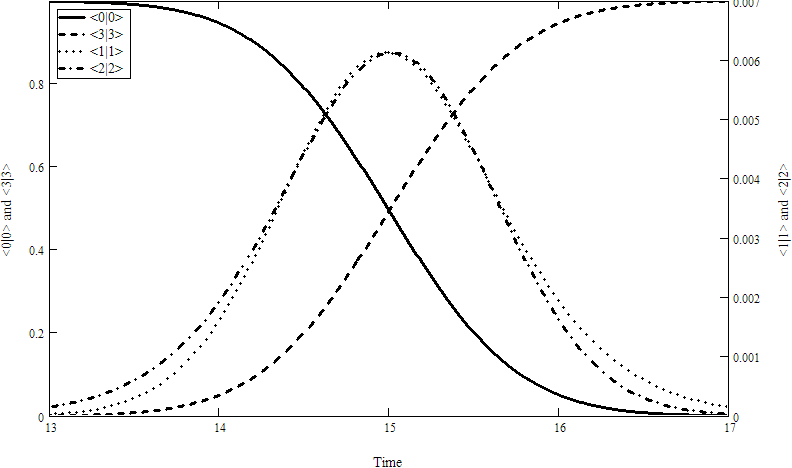
\includegraphics[width=5.00in]
{solution_3_energy_levels/solution_3_energy_levels.png}\\
\caption[Three color optimal solution]{Three color optimal solution. Occupation probability of the intermediate states $\ket{1}$ and $\ket{2}$ remain small while states $\ket{0}$ and $\ket{3}$ essentially exchange unity occupation probability in what looks like a single color $\pi$-pulse process (see figure \ref{solution one}).}
\label{solution three energy levels}
\end{figure} 
%----------------------------------------------------------------------------

%----------------------------------------------------------------------------
%----------------------------------------------------------------------------
\begin{equation}
\Phi_{intermediate}
=
\sum_i^N
P_1(t_i)
+
P_2(t_i)
\label{three int cost}
\end{equation}
%----------------------------------------------------------------------------
and $w$ is some weight factor.
%----------------------------------------------------------------------------
%----------------------------------------------------------------------------
A MathCAD program was written to minimize (\ref{three cost}) as a function of $\sigma_\alpha$, $\sigma_\beta$, $\sigma_\gamma$, $A$, $B$, $C$, $\Delta_\alpha$ and $\Delta_\gamma$. After some initial runs, some symmetries in the solutions prompted the following reduction of variables: $\sigma_\alpha=\sigma_\gamma$, $A=C$, $\Delta_\alpha=\Delta_\gamma$. Figure \ref{solution three pulses} shows the pulse sequence which minimized the cost function and figure \ref{solution three energy levels} shows the resulting motion in $\braket{\Psi}{\Psi}$.

In general, there are many local optima in the five dimensional solution space. It was found (with some exploring) that these optima generally improve with increasing amplitudes $A$, $B$, and $C$. Figure \ref{big solution three energy levels} show an example of one such solution. Note again the ``counter--intuitive'' pulse order of the first and last pulse.
%----------------------------------------------------------------------------
%----------------------------------------------------------------------------
% big_solution_3_energy_levels.tex
% by Troy Hix, April 2005
%----------------------------------------------------------------------------
\begin{figure}
\centering
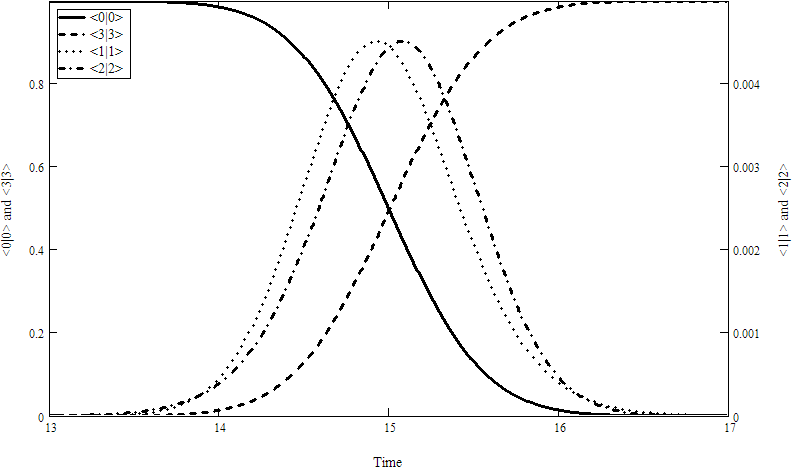
\includegraphics[width=5.00in]
{big_solution_3_energy_levels/big_solution_3_energy_levels.png}\\
\caption[Three color optimal solution - increased pulse amplitude]{Three color optimal solution - increased pulse amplitude. The local optimum ($w=10^8$) occurs when $\sigma_\alpha=\sigma_\gamma=2.19612383897$, $\sigma_\beta=4.57812933276$, $A=C=15.8819988348$ (7.524 times the area of the $\pi$--pulse), $B=101.198555496$ (99.937 times the area of the $\pi$--pulse), and $\Delta_\alpha=\Delta_\gamma=-0.93886228288$.}
\label{big solution three energy levels}
\end{figure} 
%----------------------------------------------------------------------------

%----------------------------------------------------------------------------
%----------------------------------------------------------------------------
%----------------------------------------------------------------------------

%----------------------------------------------------------------------------
%----------------------------------------------------------------------------
\section{Random excitation amplitude simulations}
It was observed in the laboratory that the dye lasers, intended for use in a demonstration experiment of these processes, exhibit relatively large ($\sim20\%$) intensity fluctuations. Here we estimate the effect of these fluctuations on the population transfer efficiency of various three color transfer schemes.
%----------------------------------------------------------------------------
\label{random sims}
%----------------------------------------------------------------------------
\subsection{Three $\pi$ pulse sequence}
% three_pi.tex
% by Troy Hix, April 2005
%----------------------------------------------------------------------------
\begin{figure}
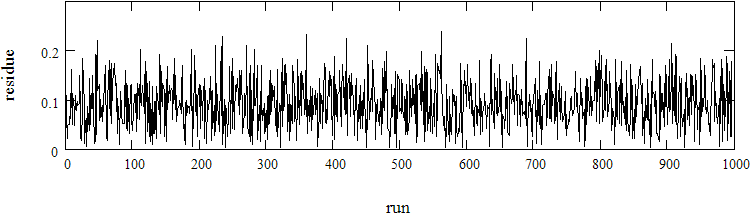
\includegraphics[width=6.00in]
{three_pi/three_pi.png}\\
\caption[Residue for runs using three $\pi$ pulses]{Residue for runs using three $\pi$ pulses. Three pulses of the form shown is figure \ref{solution one} were used at $t_\alpha=5$, $t_\beta=15$, and $t_\gamma=25$. The pulse amplitudes $A$, $B$, and $C$ varied uniformly on the interval $[-20\%,+20\%]$ for 1000 runs.}
\label{three pi}
\end{figure} 
%----------------------------------------------------------------------------
%

%----------------------------------------------------------------------------
\subsection{STIRAP sequence followed by a $\pi$ pulse}
%----------------------------------------------------------------------------
We examine a STIRAP sequence followed by pi pulse. The first two pulses are a STIRAP sequence with $t_\beta=10$, $t_\alpha=t_\beta - \Delta_\alpha = 10 + 1.26997923288$ and $A=B=10.4616402919$. The last pulse is a $\pi$ pulse with $\sigma_\gamma=2$, $t_\gamma=25$, and $C=0.737832313319$. For each run the amplitudes are selected in a uniform random fashion on the interval $[-20\%,+20\%]$ using the ``runif'' random number generator in MathCAD. Then a fourth-order Runge-Kutta fixed-step method is used to find the solution at 5001 points in the interval, and hence the residue ($\Psi_{residue}$) for each run. See figure \ref{STIRAP plus pi pulse}.
%----------------------------------------------------------------------------
%----------------------------------------------------------------------------
%----------------------------------------------------------------------------
We examine a STIRAP sequence followed by pi pulse. The first two pulses are a STIRAP sequence with $t_\beta=10$, $t_\alpha=t_\beta - \Delta_\alpha = 10 + 1.26997923288$ and $A=B=10.4616402919$. The last pulse is a $\pi$ pulse with $\sigma_\gamma=2$, $t_\gamma=25$, and $C=0.737832313319$. For each run the amplitudes are selected in a uniform random fashion on the interval $[-20\%,+20\%]$ using the ``runif'' random number generator in MathCAD. Then a fourth-order Runge-Kutta fixed-step method is used to find the solution at 5001 points in the interval, and hence the residue ($\Psi_{residue}$) for each run. See figure \ref{STIRAP plus pi pulse}.
%----------------------------------------------------------------------------
%----------------------------------------------------------------------------
%----------------------------------------------------------------------------
We examine a STIRAP sequence followed by pi pulse. The first two pulses are a STIRAP sequence with $t_\beta=10$, $t_\alpha=t_\beta - \Delta_\alpha = 10 + 1.26997923288$ and $A=B=10.4616402919$. The last pulse is a $\pi$ pulse with $\sigma_\gamma=2$, $t_\gamma=25$, and $C=0.737832313319$. For each run the amplitudes are selected in a uniform random fashion on the interval $[-20\%,+20\%]$ using the ``runif'' random number generator in MathCAD. Then a fourth-order Runge-Kutta fixed-step method is used to find the solution at 5001 points in the interval, and hence the residue ($\Psi_{residue}$) for each run. See figure \ref{STIRAP plus pi pulse}.
%----------------------------------------------------------------------------
%----------------------------------------------------------------------------
\input{figures/transfer/STIRAP_pi/STIRAP_pi.tex}
%----------------------------------------------------------------------------
%----------------------------------------------------------------------------
%----------------------------------------------------------------------------
%----------------------------------------------------------------------------
%----------------------------------------------------------------------------
%----------------------------------------------------------------------------

%----------------------------------------------------------------------------
%----------------------------------------------------------------------------
%----------------------------------------------------------------------------
%----------------------------------------------------------------------------
%----------------------------------------------------------------------------
%----------------------------------------------------------------------------

%----------------------------------------------------------------------------
%----------------------------------------------------------------------------
%----------------------------------------------------------------------------
%----------------------------------------------------------------------------
%----------------------------------------------------------------------------
%----------------------------------------------------------------------------

%----------------------------------------------------------------------------
\subsection{Three color optimal sequence}
% three_STIRAP.tex
% by Troy Hix, April 2005
%----------------------------------------------------------------------------
\begin{figure}
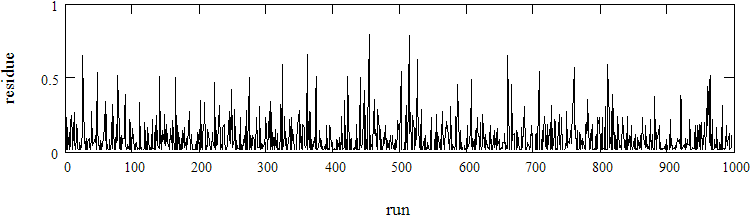
\includegraphics[width=6.00in]
{three_STIRAP/three_STIRAP.png}\\
\caption[Residue for runs using three color STIRAP]{Residue for runs using three color STIRAP. A pulse sequence of the form show in figure \ref{solution three pulses} is used here. The pulse amplitudes $A$, $B$, and $C$ varied uniformly on the interval $[-20\%,+20\%]$ for 1000 runs.}
\label{three color optimum}
\end{figure} 
%----------------------------------------------------------------------------

%----------------------------------------------------------------------------
\subsection{Histogram comparison}
% histogram.tex
% by Troy Hix, April 2005
%----------------------------------------------------------------------------
%----------------------------------------------------------------------------
\begin{figure}
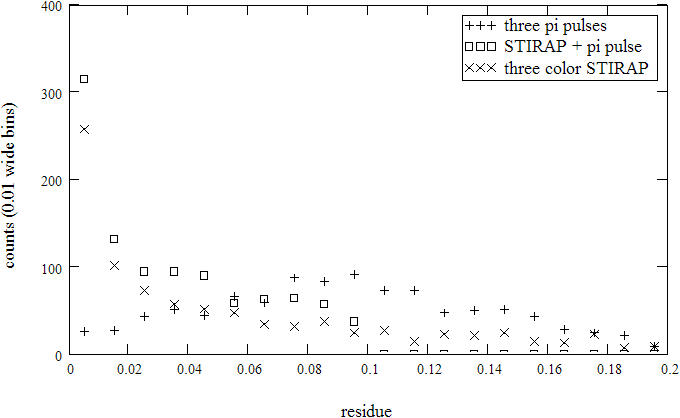
\includegraphics[width=5.00in]
{histogram/histogram.png}\\
\caption[Stochastic simulation histograms]{Stochastic simulation histograms. Notice that the three $\pi$ pulse sequence has a peak somewhere near 0.1 while the other two sequences seem peaked near zero.}
\label{histogram}
\end{figure} 
%----------------------------------------------------------------------------

%----------------------------------------------------------------------------
%----------------------------------------------------------------------------
\section{Stochastic collision model and density matrix methods}
First, we examine the effect of collision using a ``state vector'' approach assuming that the effect of collisions is to simply randomize the ``phase'' of the atom. Then we try to merge this idea with density matrix methods using a computer fit to the free parameters in a ``relaxation'' matrix. Modeling the effects of collisions in a stochastic manner (as in Section \ref{model} is computationally intensive and slow. The density matrix method is computational simple and would be preferred for further investigation into collisional effects.
\label{density section}
%----------------------------------------------------------------------------
\subsection{Collision model}
%----------------------------------------------------------------------------
\label{model}
%----------------------------------------------------------------------------
%----------------------------------------------------------------------------
%bb defines the bounding box for the pdf
%viewport defines the area of the pdf used
%in sidewaysfigure the last entry in bb moves the caption toward/away the pic
%in sidewaysfigure the second entry in bb moves the pic toward/away the caption
%----------------------------------------------------------------------------
\begin{figure}
\scalebox{0.8}[0.8]{
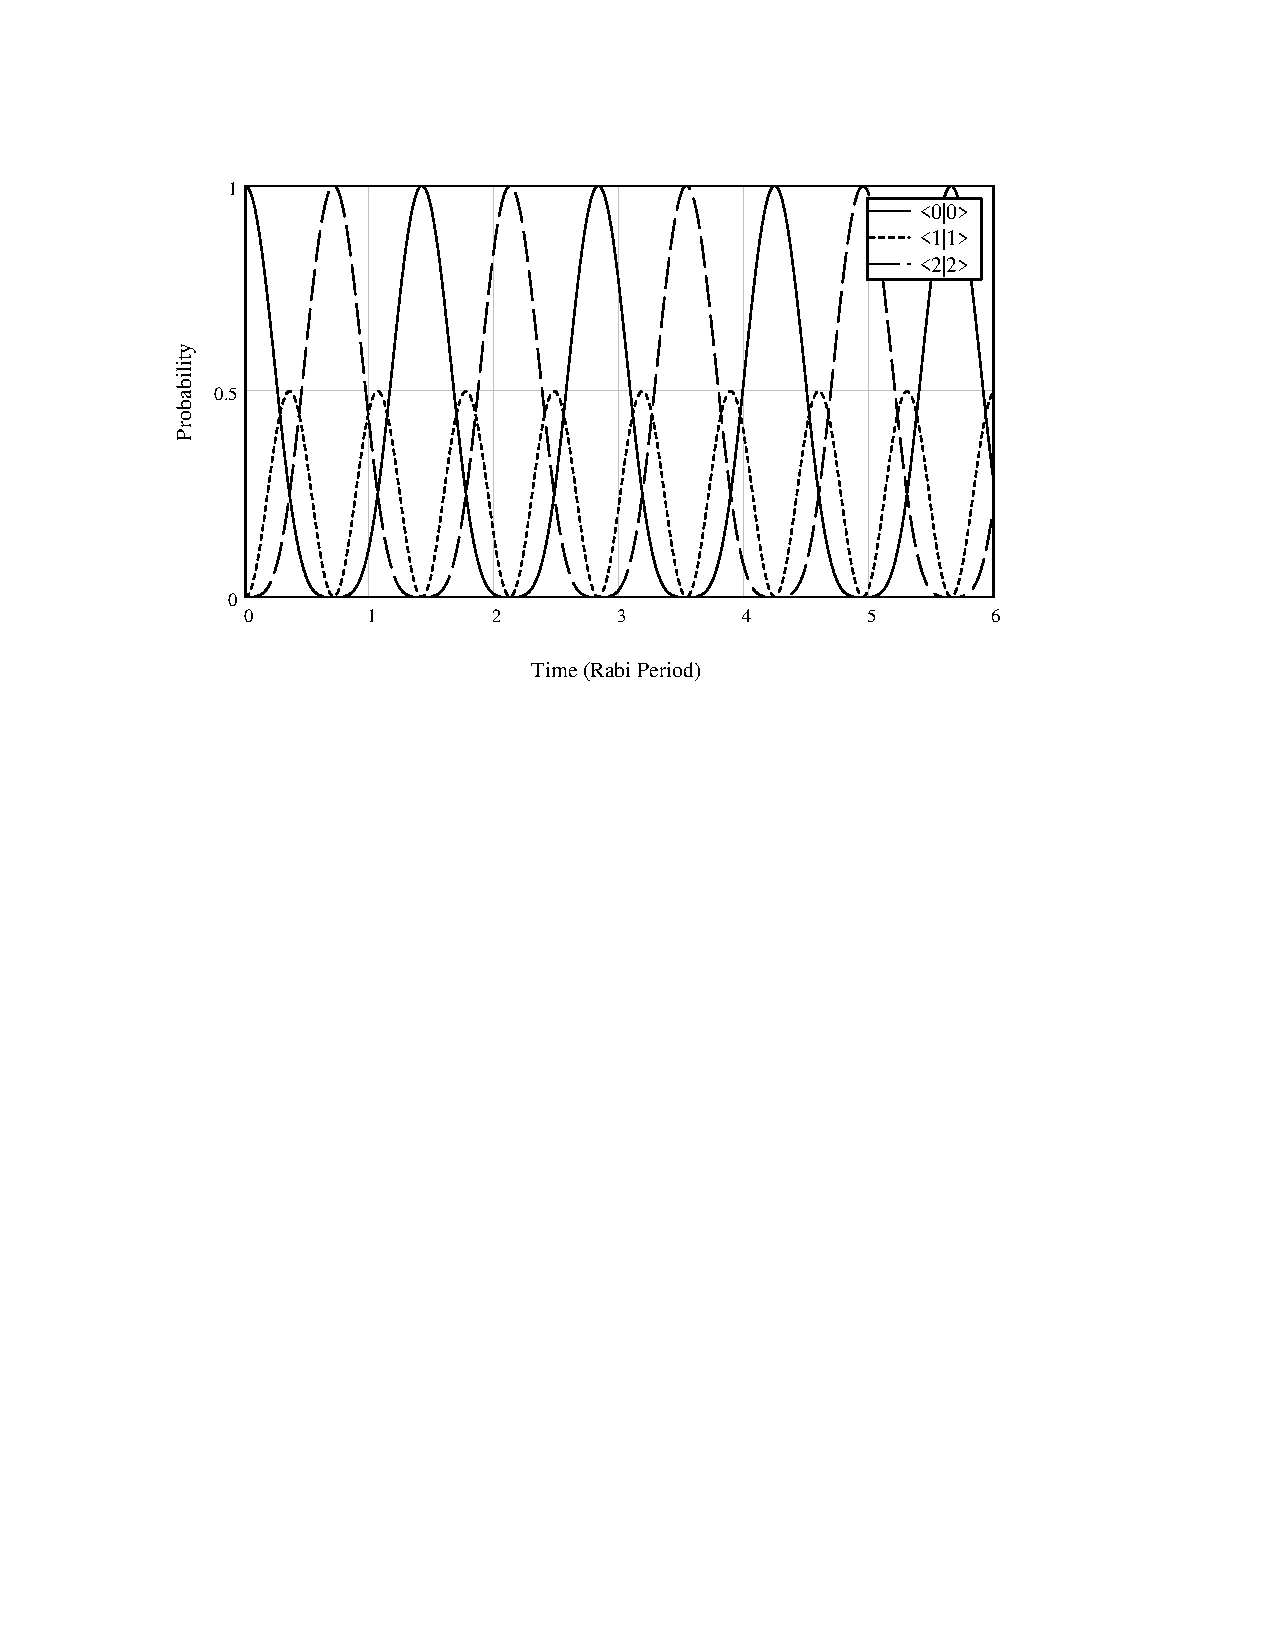
\includegraphics[bb=30 455 489 685]
{clean/clean.pdf}
}
\caption[Collisionless evolution of a three state system]{Collisionless evolution of a three state system. For this (and the following simulations) $\alpha=\beta=1$ and the time scale is the two state Rabi period associated with $\alpha$ (or $\beta$).}
\label{clean}
\end{figure}
%----------------------------------------------------------------------------

%----------------------------------------------------------------------------
%----------------------------------------------------------------------------
%bb defines the bounding box for the pdf
%viewport defines the area of the pdf used
%in sidewaysfigure the last entry in bb moves the caption toward/away the pic
%in sidewaysfigure the second entry in bb moves the pic toward/away the caption
%----------------------------------------------------------------------------
\begin{figure}
\scalebox{0.8}[0.8]{
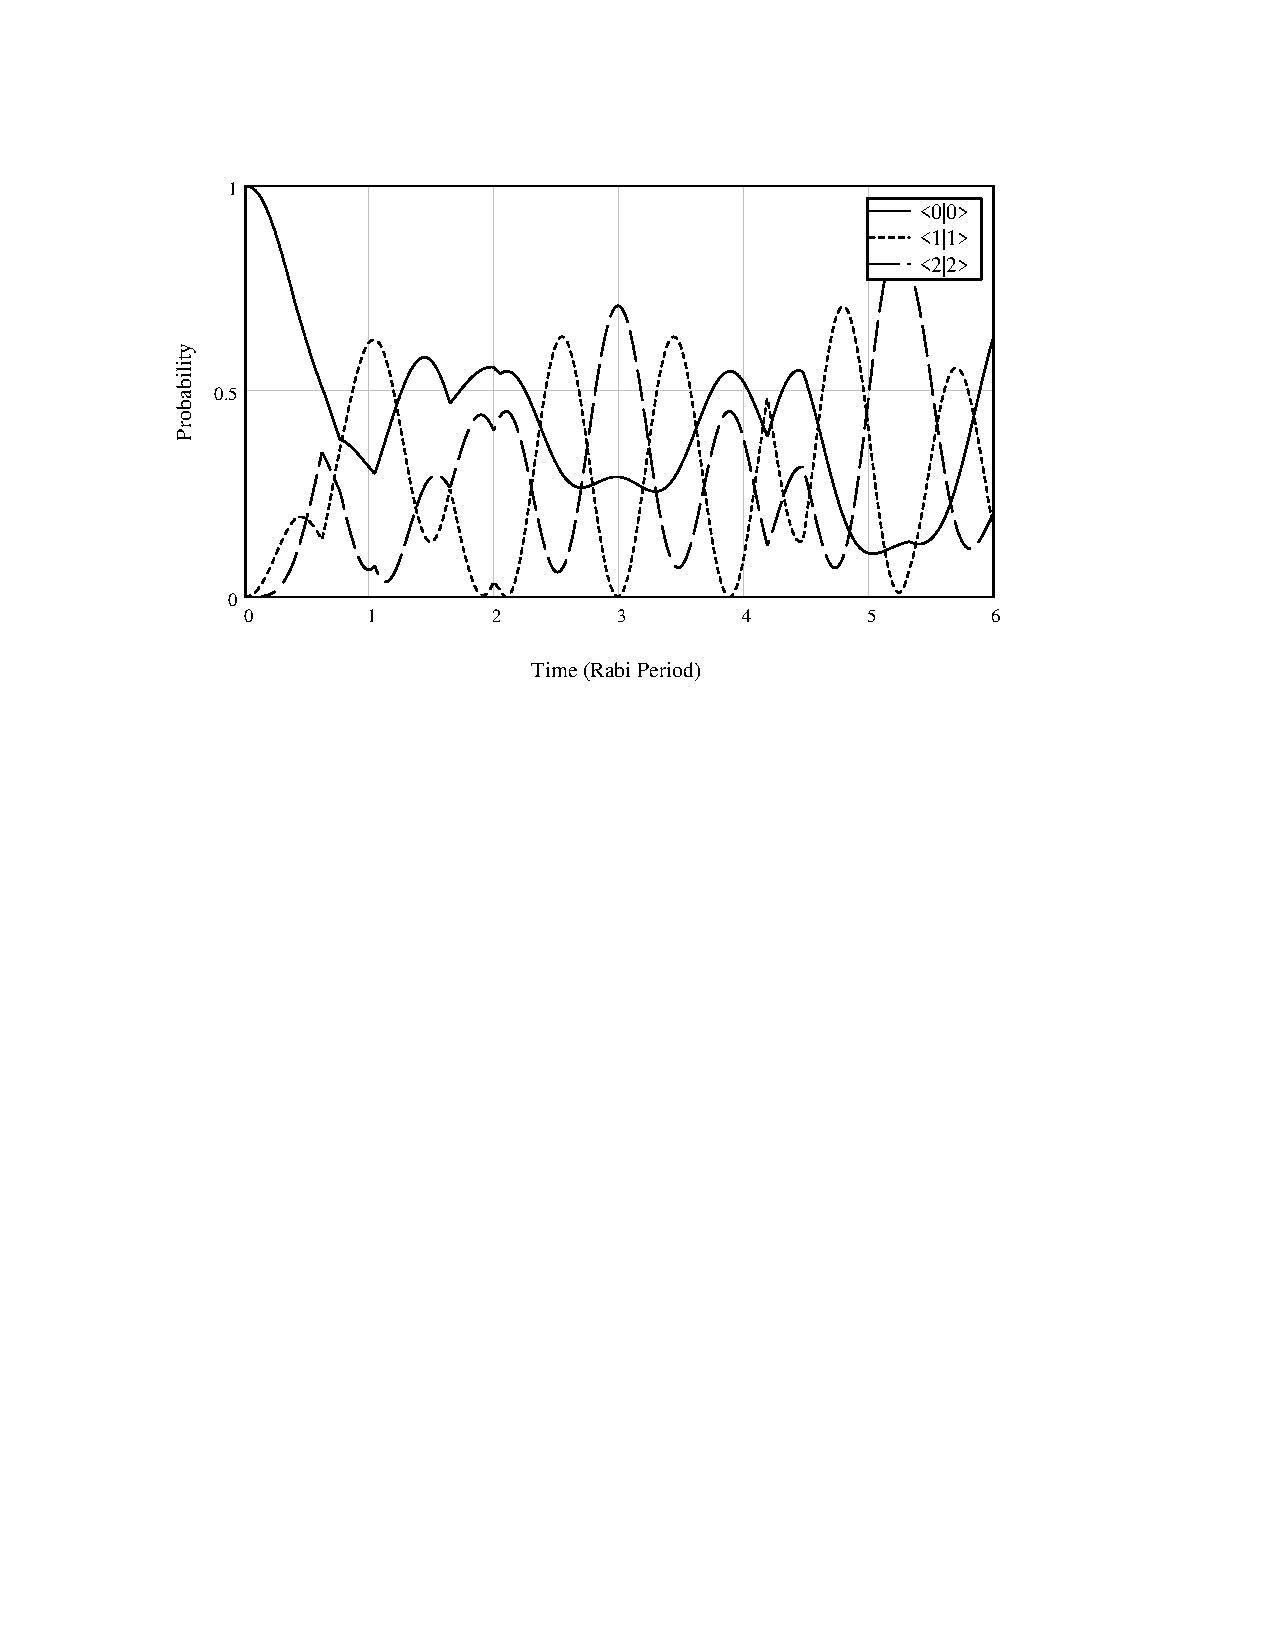
\includegraphics[bb=30 455 489 685]
{coll_1/coll_1.pdf}
}
\caption[Evolution of a three state system with collisions - example 1]{Evolution of a three state system with collisions - example 1. The probability of a collision per Rabi period is 0.5/$\pi$.}
\label{coll_1}
\end{figure}
%----------------------------------------------------------------------------

%----------------------------------------------------------------------------
%----------------------------------------------------------------------------
Reference \cite{Siegman:1986a} describes a model for the collisional effects on the quantum mechanical evolution of an atomic system. The main effect of collisions is to randomize the phase of the expansion coefficients (i.e. the ``c's'' in Equations \ref{expansion} and \ref{se}) as they evolve. (Collisions may also transfer population with relatively low probability in inelastic collisions, but this is ignored in this analysis.) This model is easy to implement in computer code written to solve Equation \ref{se}. As the code solves the equation, it is interrupted randomly. The phase of the expansion coefficients (the expansion coefficients are in general complex) are uniformly randomized on the interval $[0,2\pi)$ while leaving the magnitude intact. Then the numerical integrator picks up where in left off at the interruption, except with the new ``randomized'' expansion coefficients and continues until another ``collision'' (i.e. interruption) takes place. See Figures \ref{clean} through \ref{coll_2} for examples.

The probability of a collision per unit time is arbitrarily selected as $0.5/\pi$ in the examples shown here (there were additional runs at $0.3/\pi$). In Figure \ref{average} we see the result when one million runs are averaged together: the behavior has the appearance of damped oscillations. This behavior seems like it may be described in a cleaner way; if not with an analytic form, then with a differential equation. In the next section we develop a formal candidate.
%----------------------------------------------------------------------------
%----------------------------------------------------------------------------
%bb defines the bounding box for the pdf
%viewport defines the area of the pdf used
%in sidewaysfigure the last entry in bb moves the caption toward/away the pic
%in sidewaysfigure the second entry in bb moves the pic toward/away the caption
%----------------------------------------------------------------------------
\begin{figure}
\scalebox{0.8}[0.8]{
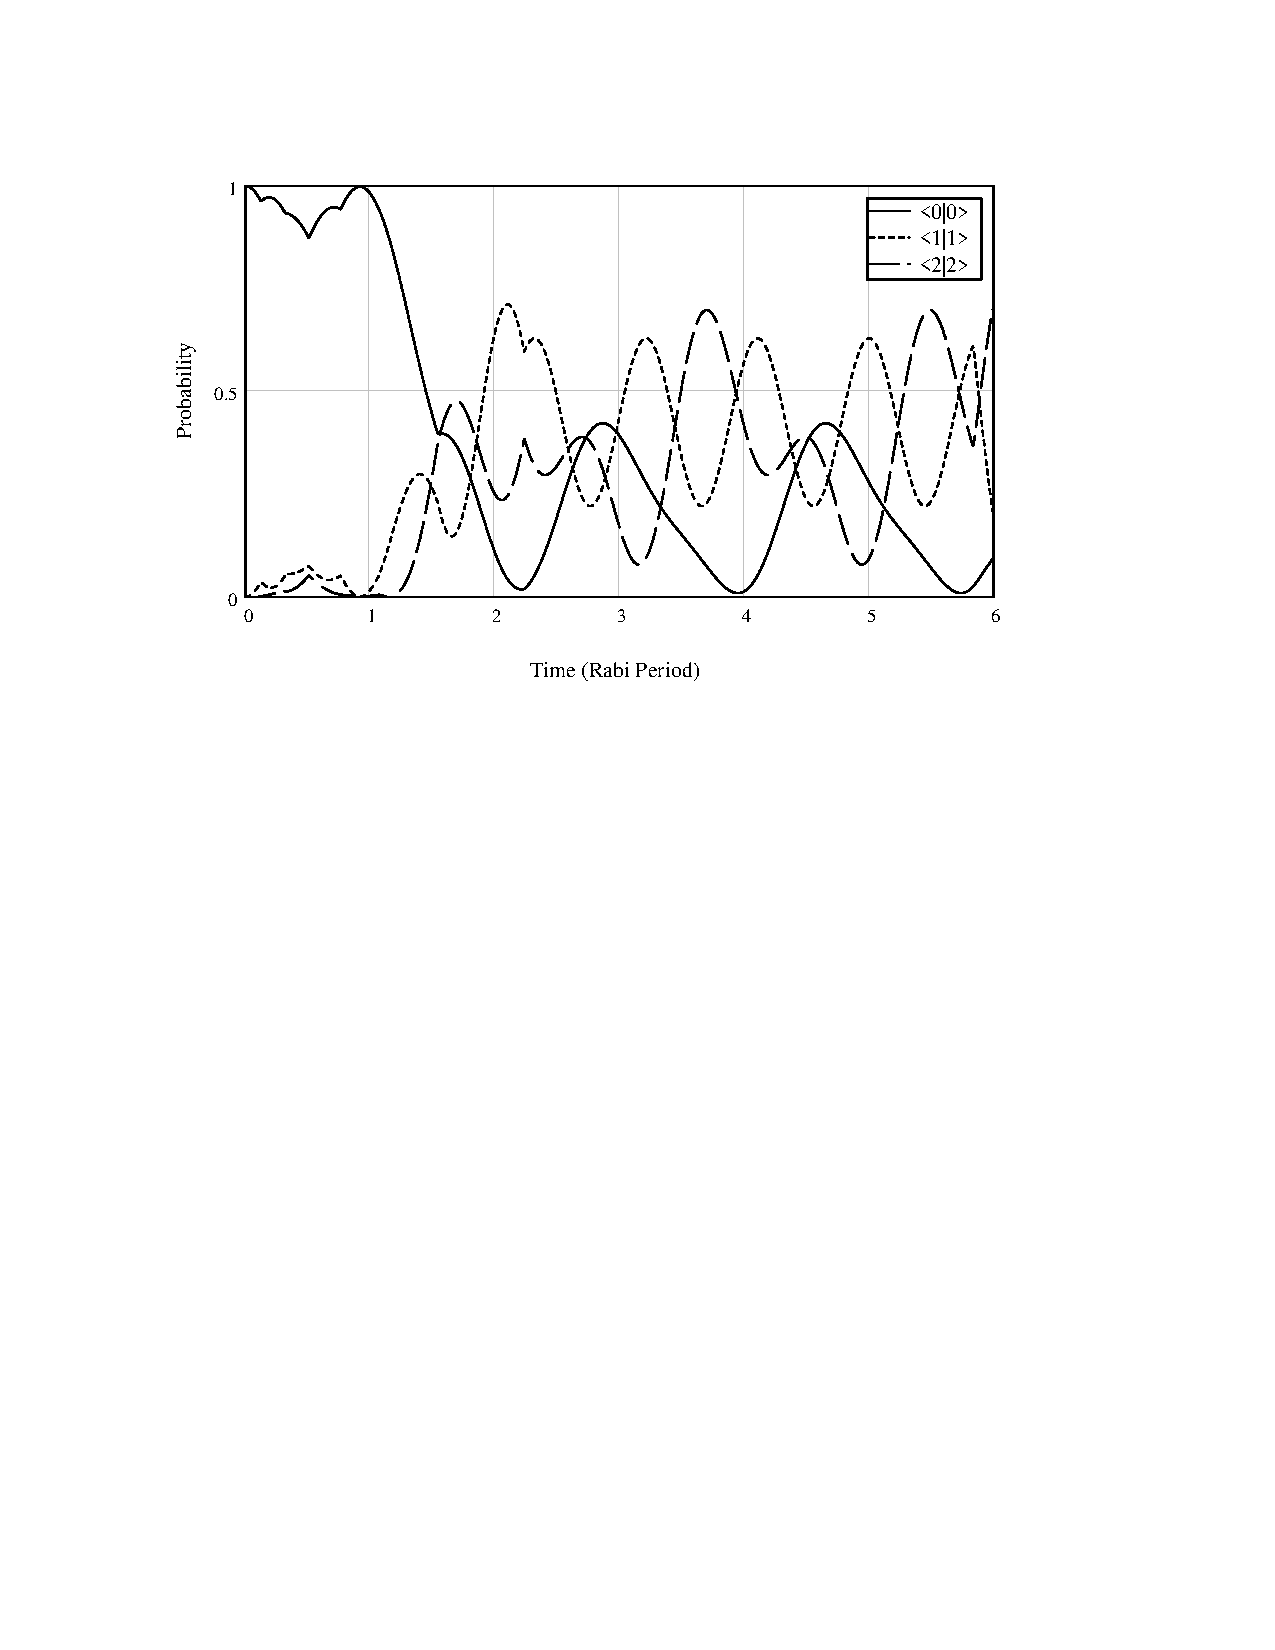
\includegraphics[bb=30 455 489 685]
{coll_2/coll_2.pdf}
}
\caption[Evolution of a three state system with collisions - example 2]{Evolution of a three state system with collisions - example 2. The probability of a collision per Rabi period is 0.5/$\pi$.}
\label{coll_2}
\end{figure}
%----------------------------------------------------------------------------

%----------------------------------------------------------------------------
%----------------------------------------------------------------------------
%----------------------------------------------------------------------------
%----------------------------------------------------------------------------
%----------------------------------------------------------------------------

%----------------------------------------------------------------------------
\subsection{Density matrix formalism}
%----------------------------------------------------------------------------
\label{density formalism}
%----------------------------------------------------------------------------
The equation of motion for the density matrix is given by the Liouville-von Neumann equation:
\begin{equation}
i \hbar \frac{\partial \rho}{\partial t}
=
[H, \rho];
\label{Liouville equation}
\end{equation}
%----------------------------------------------------------------------------
where $H$ is the Hamiltonian and $\rho$ is the density matrix. If the system of interest is not totally isolated and the degrees of freedom due to its surroundings (the so called ``heat bath'') are unobserved, then equation (\ref{Liouville equation}) may not describe the time evolution of the system \cite{Blum:1981a}. In our application, we have a target molecule (system of interest) in a ``sea'' of non--target atmospheric molecules (the ``bath'').

We introduce a \emph{relaxation} operator $\hat{R}$ \cite{Band:1991a} to parameterize the effect of the surroundings:
%----------------------------------------------------------------------------
\begin{equation}
i \frac{\partial \rho}{\partial t}
=
[H, \rho]
+
i \hat{R} \vec{\rho}.
\label{open Liouville equation}
\end{equation}
%----------------------------------------------------------------------------
If we are working in $n$ dimensional Hilbert space, the left hand side and the first two terms on the right hand side are $n\cross n$ matrices. Since the last term is in Liouville space (i.e. $\vec{\rho} = (\rho_{00}, \cdots, \rho_{nn})^{T}$ and $\hat{R}$ is a $n^2\cross n^2$ matrix) there remains a one to one correspondence between the elements of each term in the equation of motion.

Let us consider the example of a many--level system (perhaps a target molecule with its many ro-vibrational levels) where we are only concerned with a small subset of these levels -- specifically two levels (perhaps the two levels resonantly coupled with a tuned laser field). The Hamiltonian from Equation \ref{two dynamics} is:
%----------------------------------------------------------------------------
\begin{equation}
H
=
i\left(
\begin{array}{cc}
0 & \alpha \\
-\alpha & 0
\end{array}
\right).
\label{Hilbert}
\end{equation}
%----------------------------------------------------------------------------
Next we give the relaxation matrix a specific form.
%----------------------------------------------------------------------------
\begin{equation}
\hat{R}
=
\hat{R}^{ext}
+
\hat{R}^{int}
+
\hat{R}^{phase};
\label{R}
\end{equation}
%----------------------------------------------------------------------------
where $\hat{R}^{ext}$ represents the tendency of the two level subset to relax into the other levels outside the subset (external relaxation), $\hat{R}^{int}$ represents the tendency of one level in the subset to relax into another level in the subset (internal relaxation), and $\hat{R}^{phase}$ represents de--phasing resulting from the relaxation process mentioned above and/or from other sources (perhaps collisions).
%----------------------------------------------------------------------------
\begin{equation}
\hat{R}^{ext}
=
\left(
\begin{array}{cccc}
-\Gamma_{00} & 0 & 0 & 0 \\
0 & 0 & 0 & 0 \\
0 & 0 & 0 & 0 \\
0 & 0 & 0 & -\Gamma_{11} 
\end{array}
\right),
\label{decay}
\end{equation}
%----------------------------------------------------------------------------
\begin{equation}
\hat{R}^{int}
=
\left(
\begin{array}{cccc}
-\Gamma^{0}_{1} & 0 & 0 & \Gamma^{0}_{1}  \\
0 & 0 & 0 & 0 \\
0 & 0 & 0 & 0 \\
\Gamma^{1}_{0} & 0 & 0 & -\Gamma^{1}_{0} 
\end{array}
\right), \quad \mbox{and}
\label{exchange}
\end{equation}
%----------------------------------------------------------------------------
\begin{equation}
\hat{R}^{phase}
=
\left(
\begin{array}{cccc}
0 & 0 & 0 & 0 \\
0 & \gamma_{01} & 0 & 0 \\
0 & 0 & \gamma_{01} & 0 \\
0 & 0 & 0 & 0 
\end{array}
\right);
\label{dephase}
\end{equation}
%----------------------------------------------------------------------------
where $\Gamma_{ii}$ is the relaxation rate of the state $i$ to some external state, $\Gamma^i_j$ is the relaxation rate of state $i$ into state $j$, and $\gamma_{ij}$ is the relaxation rate of $\rho_{ij}$ $(i \not= j)$. $\Gamma_{ii}$ is the rate at state $i$ relaxes to some other level \emph{outside} the subset under consideration; hence if $\Gamma_{ii}\not=0$ then probability will not be conserved in equation (\ref{open Liouville equation}). $\gamma_{ij}$ is applied to only the off diagonal terms in the density matrix; thus it is the rate at which the system loses coherence.
%----------------------------------------------------------------------------
%----------------------------------------------------------------------------
%----------------------------------------------------------------------------
%----------------------------------------------------------------------------
%----------------------------------------------------------------------------
%----------------------------------------------------------------------------
%----------------------------------------------------------------------------
%----------------------------------------------------------------------------
%----------------------------------------------------------------------------
%----------------------------------------------------------------------------

Now suppose our subsystem has three levels (see Figure \ref{2 color ladder}). The Hamiltonian from Equation \ref{three dynamics} is:
%----------------------------------------------------------------------------
\begin{equation}
H
=
i\left(
\begin{array}{ccc}
0 & \alpha & 0 \\
-\alpha & 0 & \beta \\
0 & -\beta & 0
\end{array}
\right).
\label{Hilbert3}
\end{equation}
%----------------------------------------------------------------------------
Using the same definitions as in the two level case, we can write the relaxation matrix terms as
%----------------------------------------------------------------------------
\begin{equation}
\hat{R}^{ext}
=
\left(
\begin{array}{ccccccccc}
-\Gamma_{00} & 0 & 0 & 0 & 0 & 0 & 0 & 0 & 0 \\
0 & 0 & 0 & 0 & 0 & 0 & 0 & 0 & 0 \\
0 & 0 & 0 & 0 & 0 & 0 & 0 & 0 & 0 \\
0 & 0 & 0 & 0 & 0 & 0 & 0 & 0 & 0 \\
0 & 0 & 0 & 0 & -\Gamma_{11} & 0 & 0 & 0 & 0 \\
0 & 0 & 0 & 0 & 0 & 0 & 0 & 0 & 0 \\
0 & 0 & 0 & 0 & 0 & 0 & 0 & 0 & 0 \\
0 & 0 & 0 & 0 & 0 & 0 & 0 & 0 & 0 \\
0 & 0 & 0 & 0 & 0 & 0 & 0 & 0 & -\Gamma_{22}
\end{array}
\right),
\label{decay3}
\end{equation}
%----------------------------------------------------------------------------
%----------------------------------------------------------------------------
\begin{equation}
\hat{R}^{int}
=
\left(
\begin{array}{ccccccccc}
-\Gamma^{0}_{1}-\Gamma^{0}_{2} & 0 & 0 & 0 & \Gamma^{0}_{1} & 0 & 0 & 0 & \Gamma^{0}_{2} \\
0 & 0 & 0 & 0 & 0 & 0 & 0 & 0 & 0 \\
0 & 0 & 0 & 0 & 0 & 0 & 0 & 0 & 0 \\
0 & 0 & 0 & 0 & 0 & 0 & 0 & 0 & 0 \\
\Gamma^{1}_{0} & 0 & 0 & 0 & -\Gamma^{1}_{0}-\Gamma^{1}_{2} & 0 & 0 & 0 & \Gamma^{1}_{2} \\
0 & 0 & 0 & 0 & 0 & 0 & 0 & 0 & 0 \\
0 & 0 & 0 & 0 & 0 & 0 & 0 & 0 & 0 \\
0 & 0 & 0 & 0 & 0 & 0 & 0 & 0 & 0 \\
\Gamma^{2}_{0} & 0 & 0 & 0 & \Gamma^{2}_{1} & 0 & 0 & 0 & -\Gamma^{2}_{0}-\Gamma^{2}_{1}
\end{array}
\right),
\label{exchange3}
\end{equation}
%----------------------------------------------------------------------------
and
%----------------------------------------------------------------------------
\begin{equation}
\hat{R}^{phase}
=
\left(
\begin{array}{ccccccccc}
0 & 0 & 0 & 0 & 0 & 0 & 0 & 0 & 0 \\
0 & \gamma_{01} & 0 & 0 & 0 & 0 & 0 & 0 & 0 \\
0 & 0 & \gamma_{02} & 0 & 0 & 0 & 0 & 0 & 0 \\
0 & 0 & 0 & \gamma_{01} & 0 & 0 & 0 & 0 & 0 \\
0 & 0 & 0 & 0 & 0 & 0 & 0 & 0 & 0 \\
0 & 0 & 0 & 0 & 0 & \gamma_{12} & 0 & 0 & 0 \\
0 & 0 & 0 & 0 & 0 & 0 & \gamma_{02} & 0 & 0 \\
0 & 0 & 0 & 0 & 0 & 0 & 0 & \gamma_{12} & 0 \\
0 & 0 & 0 & 0 & 0 & 0 & 0 & 0 & 0 
\end{array}
\right).
\label{dephase3}
\end{equation}
%----------------------------------------------------------------------------
%----------------------------------------------------------------------------
%----------------------------------------------------------------------------
%----------------------------------------------------------------------------

%----------------------------------------------------------------------------
\subsection{Collision model parametric fit}
%----------------------------------------------------------------------------
%bb defines the bounding box for the pdf
%viewport defines the area of the pdf used
%in sidewaysfigure the last entry in bb moves the caption toward/away the pic
%in sidewaysfigure the second entry in bb moves the pic toward/away the caption
%----------------------------------------------------------------------------
\begin{figure}
\scalebox{0.7}[0.7]{
\includegraphics*[bb=75 286 643 540]
{fit/fit.pdf}
}
\caption[Gaussinan fit for a single RF beat spectral feature]{The spectral feature at 1200 MHz fits a Gaussian with a FWHM of 83 MHz. This corresponds to a Gaussian in the time domain with a FWHM of 7.5 ns. This matches the observed pulse width - implying each mode is transform limited.}
\label{fit}
\end{figure}
%----------------------------------------------------------------------------

%----------------------------------------------------------------------------
%----------------------------------------------------------------------------
\section{Conclusion}
%----------------------------------------------------------------------------
%------------------------------Broad objectives------------------------------
%----------------------------------------------------------------------------
This chapter chronicles the stages of laboratory development undergone over the past few years. The main measurements at each stage were used as a guide to develop the equipment and techniques required for demonstration of molecular control in LIDAR systems.
%----------------------------------------------------------------------------
%----------------------------------So what?----------------------------------
%----------------------------------------------------------------------------

As each stage was completed various components of the apparatus were either designed and assembled or evolved to the next generation. After the installation of the PMT at its output the monochromator served each experiment well until the recent aromatic compound measurements. The Hg pulser and Pockles cell system went through various stages of development starting with the initial tests of the Hg pulser on LED's to the integration of the system with the YAG pumped dye laser system during the fluorescence line decay measurements. The software model was tested at each stage from the familiar non-resonant HeNe LIF to pulsed resonant dye LIF. The data acquisition system was built for the first dye laser experiments and has remained relatively unchanged since then. Recently, a calibration issue with the monochromator self scan feature has prompted the need of a second generation of the data acquisition software.
%----------------------------------------------------------------------------
%---------------------------------Synthesize---------------------------------
%----------------------------------------------------------------------------
%----------------------------------------------------------------------------
%----------------------------------------------------------------------------
%----------------------------------------------------------------------------

%----------------------------------------------------------------------------
%----------------------------------------------------------------------------
